\documentclass[12pt]{scrartcl}

% packages
\usepackage[
    a4paper, total={18cm, 26cm},
    left=0.75in,
    right=0.75in,
    top=0.75in,
    bottom=0.50in,
    footskip=15pt
]{geometry}
\usepackage{lastpage}
\usepackage{graphicx} % \includegraphics
\usepackage{amsmath, esint} % math
\usepackage{steinmetz} % \phase
\usepackage{import} % \import
\usepackage{esdiff} % \diff
\usepackage{fancyhdr} % header and footer
\usepackage{listings}

\makeatletter
\def\today{%
  \two@digits{\the\day}/%
  \ifcase\month\or%
  01\or 02\or 03\or 04\or 05\or 06\or%
  07\or 08\or 09\or 10\or 11\or 12\fi/%
  \number\year%
}
\makeatother

% configs
\setlength{\parindent}{0pt}

% comandos
\renewcommand{\familydefault}{\sfdefault}
\newcommand{\un}[1]{\;\textrm{#1}}
\newcommand{\logo}{\quad \Rightarrow \quad}
\newcommand{\fase}[1]{\ensuremath{\phase{{#1}^{\circ}}}}

\newcommand*\VF[1]{\mathbf{#1}}
\newcommand*\dif{\mathop{}\!\mathrm{d}}


\begin{document}

\pagestyle{fancy}

\fancyhead{}
\fancyhead[L]{Python Aplicado a Sinais e Sistemas - PET Engenharias}
\fancyhead[R]{Data: \today}
\fancyfoot{}
\fancyfoot[R]{Pág. \thepage \; / \pageref{LastPage}}

\begin{center}
    Aluno: Raphael Henrique Braga Leivas \\[20pt]
    Email: rapha.lei8@gmail.com
\end{center}

\hrule

\section*{Atividade 4 - Capítulo 5}

O código completo usado nessa atividade se encontra no ANEXO A.

\subsection*{Exercício 1 (a)}

A função de transferência é dada por

\[ G(s) = \frac{s^{3} + 2 s^{2} + 5 s + 1}{\left(s + 1\right) \left(s + 2\right) \left(s + 3\right) \left(s + 4\right)} \]

Cuja resposta ao impulso é

\[ h(t) = - \frac{e^{- t} \theta\left(t\right)}{2} + \frac{9 e^{- 2 t} \theta\left(t\right)}{2} - \frac{23 e^{- 3 t} \theta\left(t\right)}{2} + \frac{17 e^{- 4 t} \theta\left(t\right)}{2} \]

Que possui forma de onda dada por 

\begin{figure}[h!]
	\begin{center}
    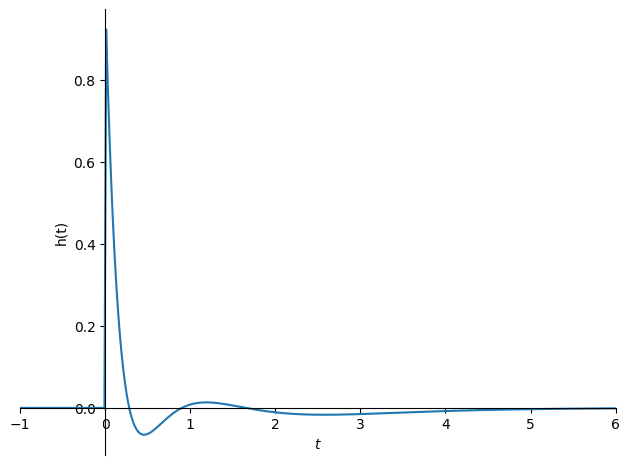
\includegraphics[width=0.8\textwidth,trim=1 1 1 1,clip]{ex1a.png}
	\end{center}
\end{figure}

Para verificar se é estável, calculamos a integral:

\[ \int_{0}^{\infty} \left| h(t) \right| \, dt = \frac{1}{24} \]

Logo, como a integral converge, temos o sistema do enunciado é BIBO estável.

\subsection*{Exercício 1 (b)}

A função de transferência é dada por

\[ G(s) = \frac{s^{3} + 5 s^{2} + 8 s + 3}{\left(s - 2\right) \left(s + 1\right) \left(s^{2} + s + 1\right)} \]

Cuja resposta ao impulso é

\[ h(t) = \left(\frac{\sqrt{3} e^{- \frac{t}{2}} \sin{\left(\frac{\sqrt{3} t}{2} \right)}}{21} - \frac{11 e^{- \frac{t}{2}} \cos{\left(\frac{\sqrt{3} t}{2} \right)}}{7}\right) \theta\left(t\right) + \frac{47 e^{2 t} \theta\left(t\right)}{21} + \frac{e^{- t} \theta\left(t\right)}{3} \]

e forma de onda 

\begin{figure}[h!]
	\begin{center}
    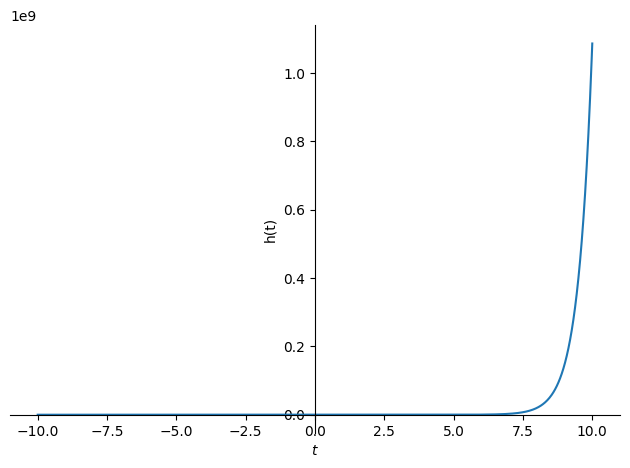
\includegraphics[width=0.8\textwidth,trim=1 1 1 1,clip]{ex1b.png}
	\end{center}
\end{figure}

Apenas olhando o gráfico, vemos que a função não tende a 0 quando $t \rightarrow \infty$.
Logo, a integral não converge e o sistema é BIBO instável.

\subsection*{Exercício 2 (a)}

Primeira coisa é encontrar a função de transferência em malha fechada
do sistema. Como $H(s) = Y(s) = 1$, temos 

\[ G(s) = \frac{P(s)}{1 + P(s)} \longrightarrow G(s) = \frac{s + 3}{s^{2} + 7 s + 11}\]

Agora plotamos os zeros e polos de $G(s)$

\begin{figure}[htp!]
	\begin{center}
    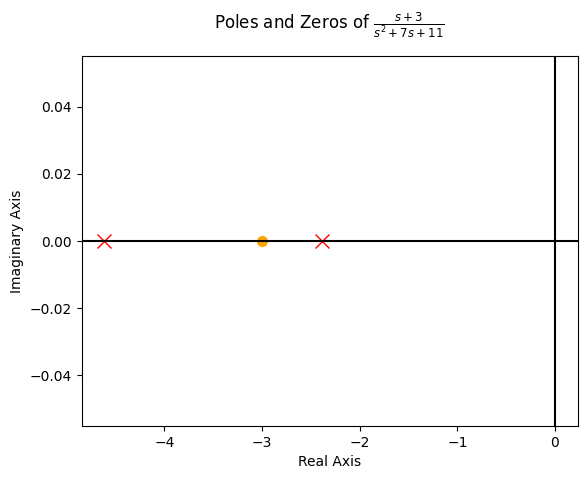
\includegraphics[width=0.8\textwidth,trim=1 1 1 1,clip]{ex2a.png}
	\end{center}
\end{figure}

Como todos os polos estão no semiplano esquerdo, temos que o sistema é BIBO estável.

\subsection*{Exercício 2 (b)}

Como $H(s) = Y(s) = 1$, temos 

\[ G(s) = \frac{P(s)}{1 + P(s)} \longrightarrow G(s) = \frac{s + 1}{s^{2} + 2 s - 5} \]

Agora plotamos os zeros e polos de $G(s)$

\begin{figure}[htp!]
	\begin{center}
    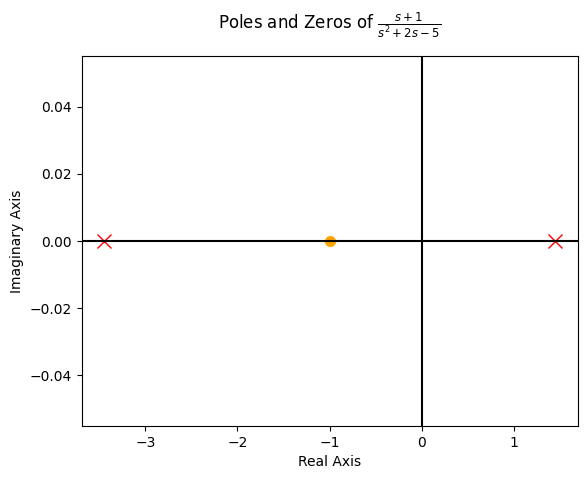
\includegraphics[width=0.8\textwidth,trim=1 1 1 1,clip]{ex2b.png}
	\end{center}
\end{figure}

Como temos pelo menos um polo no semiplano direito, temos que o sistema é BIBO instável.

\newpage

\section*{ANEXO A - Código}

\begin{lstlisting}[language=Python, breaklines=true, basicstyle=\scriptsize]
    # %%
    import numpy as np
    import matplotlib.pyplot as plt
    from sympy import *
    from sympy.physics.control.control_plots import pole_zero_plot
    from sympy.physics.control.control_plots import bode_plot
    from sympy.physics.control.lti import TransferFunction
    from sympy import oo

    # %%
    ## Exercicio 1
    t, s = symbols('t, s')
    c, C = symbols('c C', cls = Function)

    num1A = s**3 + 2*s**2 + 5*s + 1
    den1A = (s + 1) * (s + 2) * (s + 3) * (s+4)

    num1B = s**3 + 5*s**2 + 8*s + 3
    den1B = (s - 2) * (s + 1) * (s**2 + s + 1)

    print(latex(num1B / den1B))

    ht1A = inverse_laplace_transform(num1A / den1A, s, t, noconds=True)
    ht1B = inverse_laplace_transform(num1B / den1B, s, t, noconds=True)

    print(latex(ht1B))

    plot(ht1B, ylabel="h(t)")


    # %%
    convergence = integrate(ht1A, (t, 0, oo))
    print(latex(convergence))

    # %%
    # Exercicio 2
    Ps2A = (s + 3) / ((s + 2) * (s + 4))
    Gs2A = cancel(Ps2A / (1 + Ps2A))

    Ps2B = (s + 1) / ((s - 2) * (s + 3))
    Gs2B = cancel(Ps2B / (1 + Ps2B))

    print(latex(Gs2B))

    # extrai o numerador e denominador
    num, den = fraction(Gs2B)
    ft1 = TransferFunction(num, den, s)
    pole_zero_plot(ft1, pole_color="red", grid=False)
\end{lstlisting}

\end{document}